% This is a LaTeX thesis template for University of Sydney.
% to be used with Rmarkdown
% Emi Tanaka is responsible for this modified template.
% The original template is by Rob J Hyndman for students in Monash University.
% Version: 28 July 2018

\documentclass{sydneythesis}

%%%%%%%%%%%%%%%%%%%%%%%%%%%%%%%%%%%%%%%%%%%%%%%%%%%%%%%%%%%%%%%
% Add any LaTeX packages and other preamble here if required
%%%%%%%%%%%%%%%%%%%%%%%%%%%%%%%%%%%%%%%%%%%%%%%%%%%%%%%%%%%%%%%

\author{Mauricio Mardones}
\title{Krill dynamics population and fishery along Wester Antartic Peninsula}
\degrees{B.Sc. (Hons), Universidad de Concepción}
\def\country{Chile}
\def\department{CIGA}
\def\university{Universidad de Magallanes}
\def\degreetitle{Doctorate}
\def\logo{figures/logoUMAG.jpg}
% Add subject and keywords below
\hypersetup{
     pdfsubject={Integrated model},
     pdfkeywords={Fisheries, population dynamics, Stock assessment, climate change},
     pdfauthor={Mauricio Mardones},
     pdftitle={Krill dynamics population and fishery along Wester Antartic Peninsula},
     pdfproducer={Bookdown with LaTeX}
}


\bibliography{thesisrefs}

\begin{document}

\pagenumbering{roman}

\titlepage

{\setstretch{1.2}\sf\tighttoc\doublespacing}

\hypertarget{agradecimientos}{%
\chapter*{Agradecimientos}\label{agradecimientos}}
\addcontentsline{toc}{chapter}{Agradecimientos}

Generally anyone that helped you in your research journey should be acknowledged here.

Large credit of this thesis template goes to Rob J Hyndman. His original template can be found at his \href{https://github.com/robjhyndman/MonashThesis}{github repositary}.

\hypertarget{statement-of-originality}{%
\chapter*{Statement of Originality}\label{statement-of-originality}}
\addcontentsline{toc}{chapter}{Statement of Originality}

This is to certify that the intellectual content of this thesis is the product of my own work and that all the assistance received in preparing this thesis and sources have been acknowledged.

\emph{This statement is not needed for Honours Thesis.}

\vspace*{2cm}\par\authorname

\hypertarget{preface}{%
\chapter*{Preface}\label{preface}}
\addcontentsline{toc}{chapter}{Preface}

The material in Chapter \ref{ch:intro} has been submitted to the journal \emph{Journal of Impossible Results} for possible publication.

The contribution in Chapter \ref{ch:litreview} of this thesis was presented in the International Symposium on Nonsense held in Dublin, Ireland, in July 2015.

\emph{This section is not necessary for Honours Thesis.}

\hypertarget{abstract}{%
\chapter*{Abstract}\label{abstract}}
\addcontentsline{toc}{chapter}{Abstract}

The abstract is a summary of the whole thesis. Typically this section would have about 250-350 words. Check the rules of your School or University.

\clearpage\pagenumbering{arabic}\setcounter{page}{0}

\hypertarget{ch:intro}{%
\chapter{Introduction}\label{ch:intro}}

This is where you introduce the main ideas of your thesis, and an overview of the context and background.

Later chapters should be divided into coherent pieces describing your analysis. The final chapter should provide some concluding remarks, discussion, ideas for future research, and so on. Appendixes can contain additional material that don't fit into any chapters, but that you want to put on record. For example, additional tables, output, etc.

\hypertarget{rmarkdown}{%
\section{Rmarkdown}\label{rmarkdown}}

In this template, the rest of the chapter shows how to use Rmarkdown. The big advantage of using Rmarkdown is that it allows you to include your R code directly into your thesis, to ensure there are no errors in copying and pasting, and that everything is reproducible. It also helps you stay better organized.

For details on using \emph{R Markdown} see \url{http://rmarkdown.rstudio.com}.

\hypertarget{data}{%
\section{Data}\label{data}}

Included in this template is a file called \texttt{sales.csv}. This contains quarterly data on Sales and Advertising budget for a small company over the period 1981--2005. It also contains the GDP (gross domestic product) over the same period. All series have been adjusted for inflation. We can load in this data set using the following command:

\begin{Shaded}
\begin{Highlighting}[]
\NormalTok{sales }\OtherTok{\textless{}{-}} \FunctionTok{ts}\NormalTok{(}\FunctionTok{read.csv}\NormalTok{(}\StringTok{"data/sales.csv"}\NormalTok{)[,}\SpecialCharTok{{-}}\DecValTok{1}\NormalTok{], }\AttributeTok{start=}\DecValTok{1981}\NormalTok{, }\AttributeTok{frequency=}\DecValTok{4}\NormalTok{)}
\end{Highlighting}
\end{Shaded}

Any data you use in your thesis can go into the data directory. The data should be in exactly the format you obtained it. Do no editing or manipulation of the data outside of R. Any data munging should be scripted in R and form part of your thesis files (possibly hidden in the output).

\hypertarget{figures}{%
\section{Figures}\label{figures}}

Figure \ref{fig:deaths} shows time plots of the data we just loaded. Notice how figure captions and references work. Chunk names can be used as figure labels with \texttt{fig:} prefixed. Never manually type figure numbers, as they can change when you add or delete figures. This way, the figure numbering is always correct.

\begin{figure}
\centering
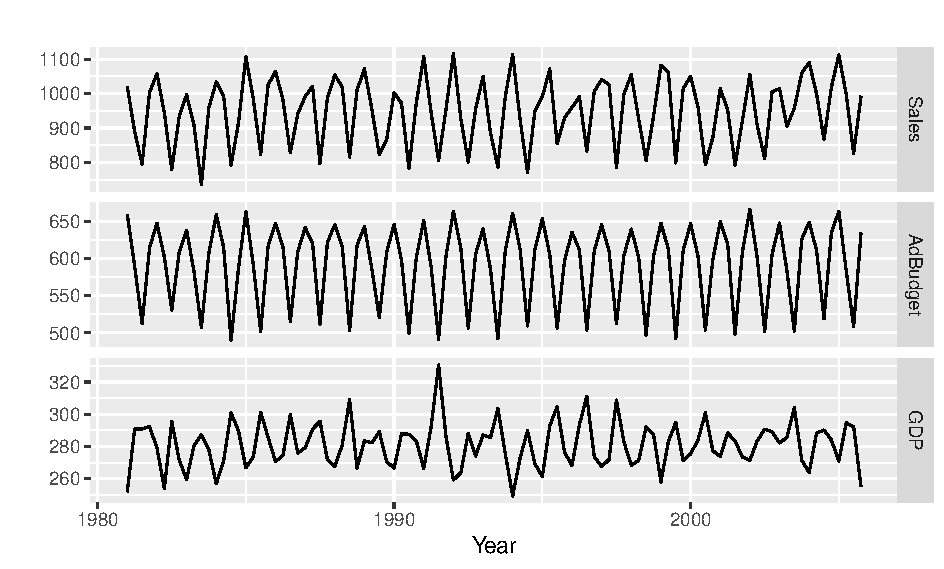
\includegraphics{thesis_files/figure-latex/deaths-1.pdf}
\caption{\label{fig:deaths}Quarterly sales, advertising and GDP data.}
\end{figure}

\hypertarget{results-from-analyses}{%
\section{Results from analyses}\label{results-from-analyses}}

We can fit a dynamic regression model to the sales data.

If \(y_t\) denotes the sales in quarter \(t\), \(x_t\) denotes the corresponding advertising budget and \(z_t\) denotes the GDP, then the resulting model is:
\begin{equation}
  y_t - y_{t-4} = \beta (x_t-x_{t-4}) + \gamma (z_t-z_{t-4}) + \theta_1 \varepsilon_{t-1} + \Theta_1 \varepsilon_{t-4} + \varepsilon_t
\end{equation}
where

\hypertarget{tables}{%
\section{Tables}\label{tables}}

Again, notice the use of labels and references to automatically generate table numbers. In this case, we need to generate the label ourselves.

The \texttt{knitLatex} package is useful for generating tables from R output. Other packages can do similar things including the \texttt{kable} function in \texttt{knitr} which is somewhat simpler but you have less control over the result. If you use \texttt{knitLatex} to generate tables, don't forget to include \texttt{results="asis"} in the chunk settings.

\hypertarget{ch:litreview}{%
\chapter{Literature Review}\label{ch:litreview}}

This chapter contains a summary of the context in which your research is set.

Imagine you are writing for your fellow PhD students. Topics that are well-known to them do not have to be included here. But things that they may not know about should be included.

Resist the temptation to discuss everything you've read in the last few years. And you are not writing a textbook either. This chapter is meant to provide the background necessary to understand the material in subsequent chapters. Stick to that.

You will need to organize the literature review around themes, and within each theme provide a story explaining the development of ideas to date. In each theme, you should get to the point where your ideas will fit in. But leave your ideas to later chapters. This way it is clear what has been done beforehand, and what new contributions you are making to the research field.

All citations should be done using markdown notation as shown below. This way, your bibliography will be compiled automatically and correctly.

\hypertarget{sec:expsmooth}{%
\section{Exponential Smoothing}\label{sec:expsmooth}}

Exponential smoothing was originally developed in the late 1950s \autocite{Brown59,Brown63,Holt57,Winters60}. Because of their computational simplicity and interpretability, they became widely used in practice.

Empirical studies by \textcite{MH79} and \textcite{Metal82} found little difference in forecast accuracy between exponential smoothing and ARIMA models. This made the family of exponential smoothing procedures an attractive proposition \autocite[see][]{CKOS01}.

The methods were less popular in academic circles until \textcite{OKS97} introduced a state space formulation of some of the methods, which was extended in \textcite{HKSG02} to cover the full range of exponential smoothing methods.

\hypertarget{ch:litreview2}{%
\chapter{Literature Review 2}\label{ch:litreview2}}

This chapter contains a summary of the context in which your research is set.

Imagine you are writing for your fellow PhD students. Topics that are well-known to them do not have to be included here. But things that they may not know about should be included.

Resist the temptation to discuss everything you've read in the last few years. And you are not writing a textbook either. This chapter is meant to provide the background necessary to understand the material in subsequent chapters. Stick to that.

You will need to organize the literature review around themes, and within each theme provide a story explaining the development of ideas to date. In each theme, you should get to the point where your ideas will fit in. But leave your ideas to later chapters. This way it is clear what has been done beforehand, and what new contributions you are making to the research field.

All citations should be done using markdown notation as shown below. This way, your bibliography will be compiled automatically and correctly.

\hypertarget{sec:expsmooth2}{%
\section{Exponential Smoothing2}\label{sec:expsmooth2}}

Exponential smoothing was originally developed in the late 1950s \autocite{Brown59,Brown63,Holt57,Winters60}. Because of their computational simplicity and interpretability, they became widely used in practice.

Empirical studies by \textcite{MH79} and \textcite{Metal82} found little difference in forecast accuracy between exponential smoothing and ARIMA models. This made the family of exponential smoothing procedures an attractive proposition \autocite[see][]{CKOS01}.

The methods were less popular in academic circles until \textcite{OKS97} introduced a state space formulation of some of the methods, which was extended in \textcite{HKSG02} to cover the full range of exponential smoothing methods.

\appendix

\hypertarget{additional-stuff}{%
\chapter{Additional stuff}\label{additional-stuff}}

You might put some computer output here, or maybe additional tables.

Note that \texttt{\textbackslash{}appendix} must appear before your first appendix although this is not required for other appendices.

\chapter{Linear Mixed Model}\label{lmm}

The extension to the linear models is the linear mixed models. A general form for the linear mixed model is given by
\begin{equation}
\boldsymbol{y} = \boldsymbol{X}\boldsymbol{\tau} + \boldsymbol{Z}\boldsymbol{u} + \boldsymbol{e} \label{eq:lmm}
\end{equation}
where \(\boldsymbol{y}\) is the \(n\times 1\) vector of observations on the trait (or response) of interest, \(\boldsymbol{\tau}\) is a \(p \times 1\) vector of fixed effects, \(\boldsymbol{u}\) is a \(q \times 1\) vector of random effects, \(\boldsymbol{X}\) and \(\boldsymbol{Z}\) are associated (known) design matrices specifying the factors and covariates (explanatory variables) with corresponding fixed and random effects vector respectively, and \(\boldsymbol{e}\) is the \(n\times 1\) vector of errors. We assume that rank of \(\boldsymbol{X}\) is \(p_0 < p\) (i.e.~non-full rank).

To complete the
specification, we assume that the joint distribution of \((\boldsymbol{u}, \boldsymbol{e})\) is
\[ \begin{bmatrix}
\boldsymbol{u} \\
\boldsymbol{e} 
\end{bmatrix}
\sim N \left( 
\begin{bmatrix}
\boldsymbol{0} \\
\boldsymbol{0} 
\end{bmatrix}, 
\begin{bmatrix}
\boldsymbol{G} & \boldsymbol{0} \\
\boldsymbol{0} & \boldsymbol{R} 
\end{bmatrix}
\right)
\]
where \(\boldsymbol{G}(\boldsymbol{\kappa_G})\) and \(\boldsymbol{R}(\boldsymbol{\kappa_R})\) are covariance matrices which depend on vectors \(\boldsymbol{\kappa_G}\) and \(\boldsymbol{\kappa_R}\) respectively; and \(\theta\) is the global scale parameter.
We let \(\boldsymbol{\kappa} = (\boldsymbol{\kappa_G}^\top, \boldsymbol{\kappa_R}^\top)^\top\) denote the complete vectors of variance parameters.

It follows that \(\boldsymbol{y} \sim N(\boldsymbol{X\tau}, \boldsymbol{V})\) where \(\boldsymbol{V} = \boldsymbol{ZGZ}^\top + \boldsymbol{R}\) where \(\boldsymbol{V}=\boldsymbol{V}(\boldsymbol{\kappa})\).

\printbibliography[heading=bibintoc]



\end{document}
